\documentclass{article}
\usepackage{graphicx} % Required for inserting images
\usepackage{float}
\title{Visual Bach}
\author{ }
\date{5 Minuten  vor Abgabefrist, 2026}

\begin{document}

\maketitle

\section{Wasserkocher Metheode}
\paragraph{}
Die Musikstücke liegen nicht nur als Notenblätter vor, sondern sind auch als Audiodateien verfügbar. In diesem Fall kann man anstatt spezifischer Methoden für die ML-Musikanalyse Methoden der Bildverarbeitung nutzen.
\\


\subsection{CQT aka Constant-Q Transform}
Die CQT ist eine Modifikation der Fourier-Transformation, die durch eine logarithmische Frequenzskala die Daten für das menschliche Verständnis besser repräsentiert.

\\
So sehen nach der CQT zwei klassische Musikstücke aus dem Maestro-Datensatz aus:
\begin{figure}[h] 
    \centering
    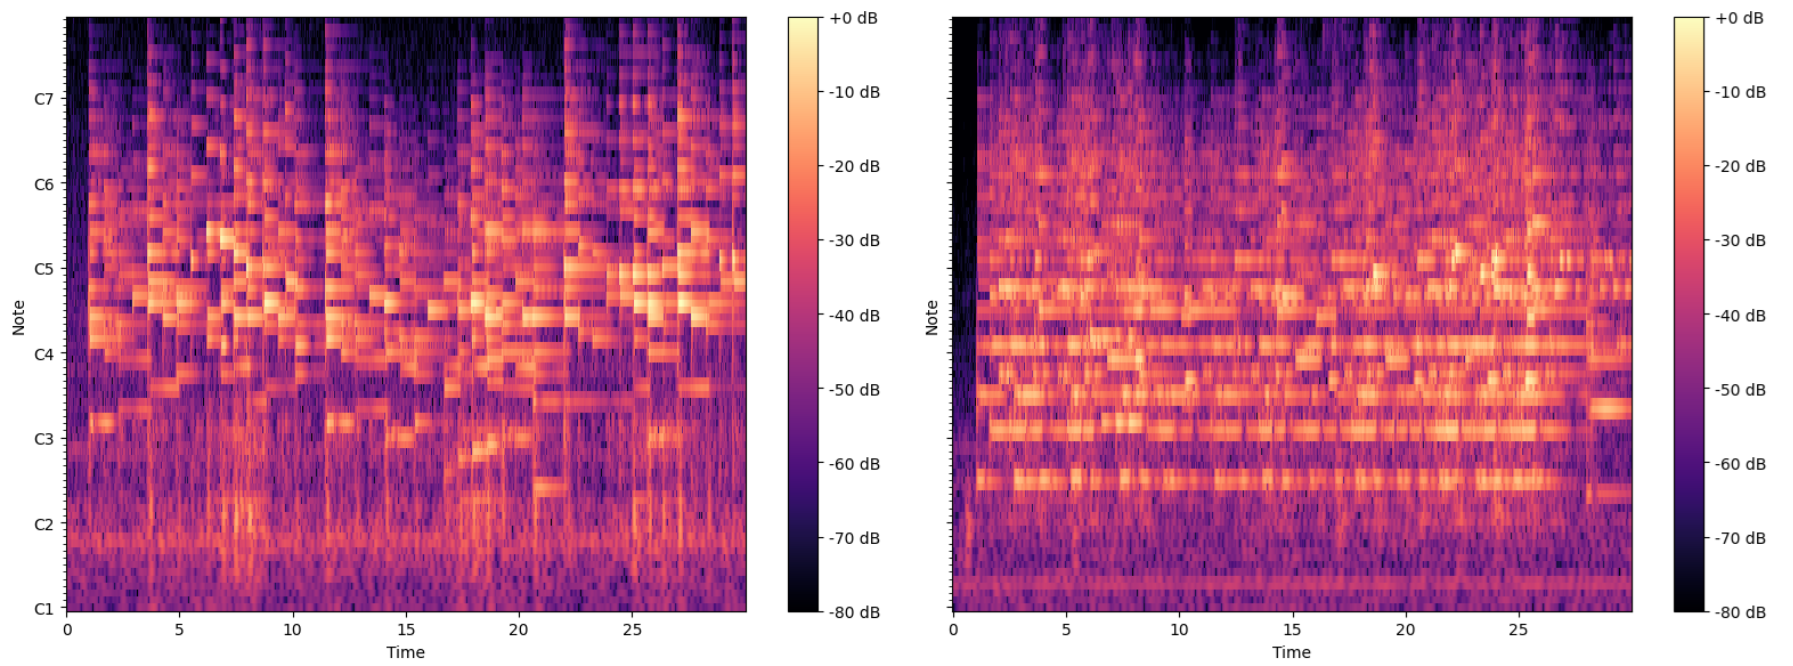
\includegraphics[width=1\textwidth]{CQT.png}
  
    \label{fig:my_image}
\end{figure}


\\ 

Und so sieht nach der CQT "Bohemian Rhapsody" von Queen aus:

\begin{figure}[H] 
    \centering
    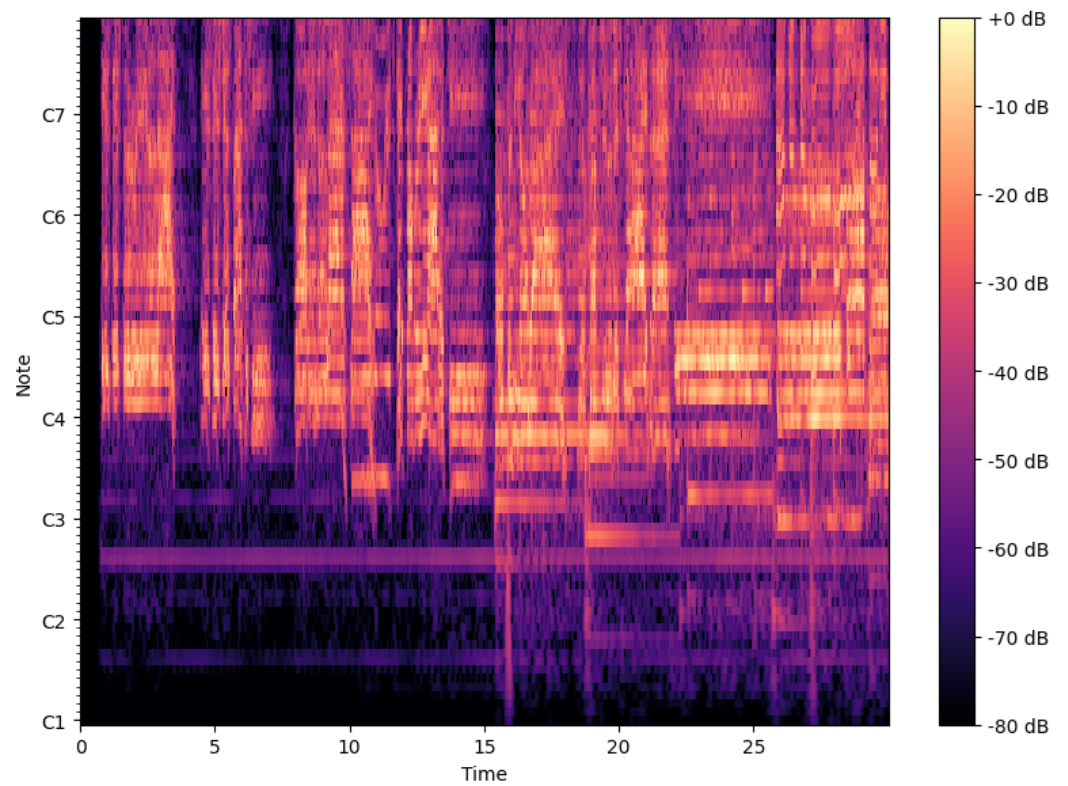
\includegraphics[width=1\textwidth]{CQueenT.png}
    \caption{\textit{Can you find a silhouette of a man?}}
    \label{fig:my_image}
\end{figure}

\subsection{Harmonie und Rhythmus}

Folgende Modellarchitektur stammt von Thomas Lidy und Alexander Schindler: „CQT-based Convolutional Neural Networks for Audio Scene Classification.“ DCASE, 2016.
\begin{figure}[H] 
    \centering
    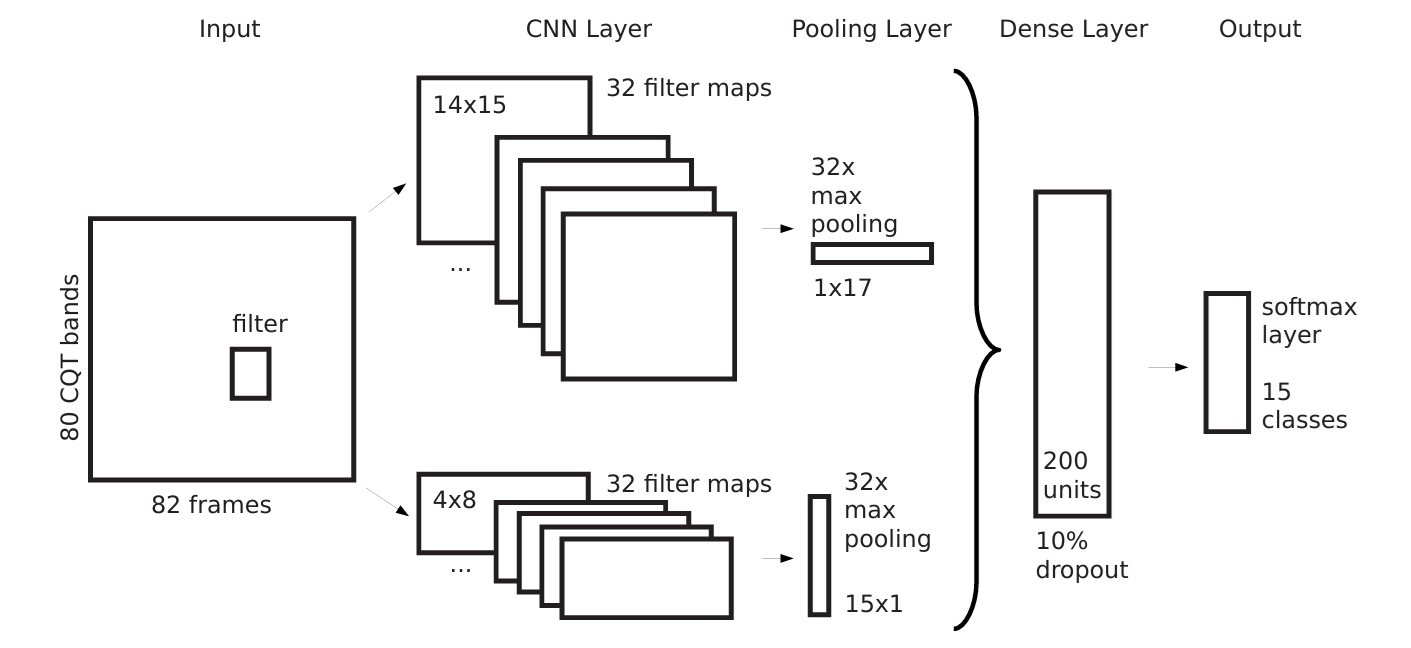
\includegraphics[width=1\textwidth]{HR.png}
    \caption{CNN Architektur}
    \label{fig:my_image}
\end{figure}

Sie wurde auf Lärm an unterschiedlichen öffentlichen Orten angewandt. Anstatt 1 Sekunde Audio zu nehmen, was 82 Frames ergibt, nehmen wir 3, 5 und 10 Sekunden.

\paragraph{}Die einzige Änderung, die in die obige Architektur eingeführt wurde, waren Max-Pooling-Schichten zu Beginn des Modells und nach der CNN-Schicht.

Im Folgenden sind die Ergebnisse aufgeführt, die mit 10.000 Intervallen aus klassischen Musikstücken aus dem Maestro-Datensatz, die 14 verschiedene Komponisten umfassen, erzielt wurden.
    
\begin{table}[h]
    \centering % This centers the table horizontally
    \caption{Genauigkeit des Objekterkennungsmodells}
    \label{tab:model_comparison}
    % Changed from 5 columns to 4 columns to match your data
    \resizebox{0.9\textwidth}{!}{% Resizes table to 80% of text width
        \begin{tabular}{|l|c|c|c|}
            \hline
            \textbf{} & \textbf{3 Sek.} & \textbf{5 Sek.} & \textbf{10 Sek.} \\ \hline
            Max pooling & 0.2570 (23.8k Total params) & 0.3060 (5.9M) & 0.2715 (12.2M) \\ \hline
            Global Average Pooling & 0.2685 (4M) & 0.3055 (23.8k) & 0.3435 (23.8k) \\ \hline
        \end{tabular}
    }
\end{table}

\subsection{Objekterkennungsmodell}
Jetzt versuchen wir eine neue CNN-Architektur, aber ignorieren die Tatsache, dass wir mit Musik arbeiten. Wenden wir ein Objekterkennungsmodell an.
\begin{figure}[H] 
    \centering
    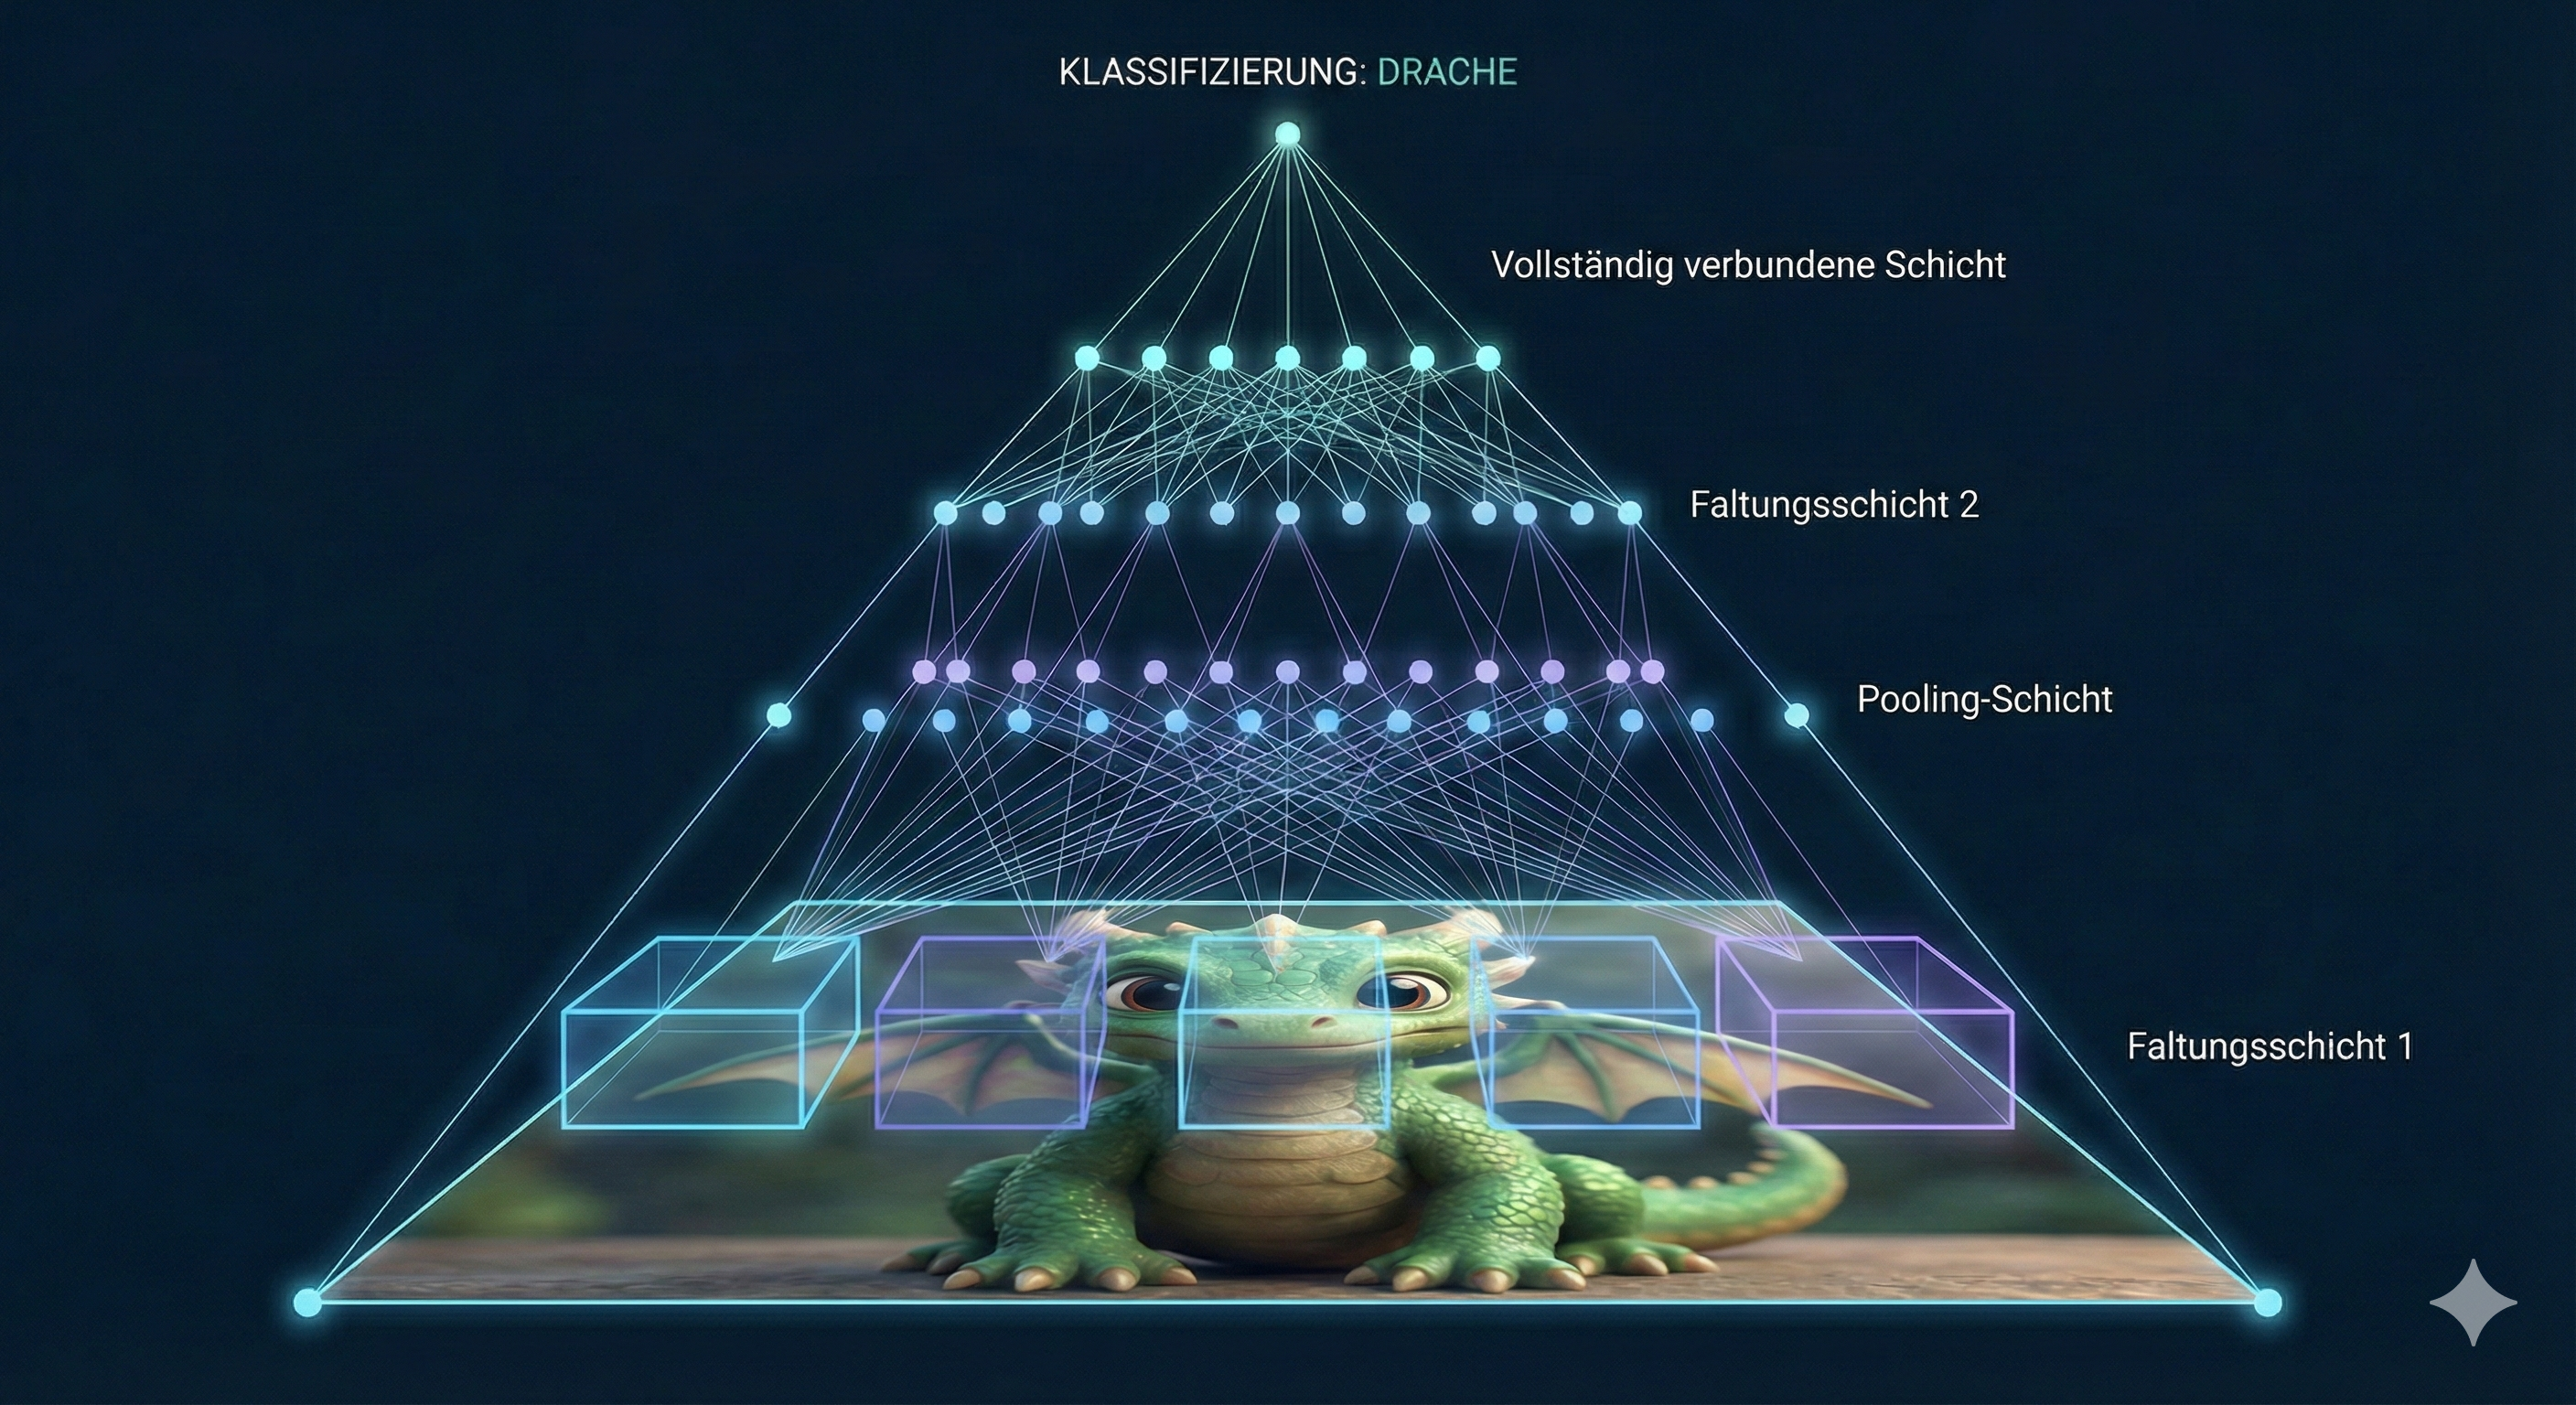
\includegraphics[width=0.8\textwidth]{dragon.png}
    
    \label{fig:my_image}
\end{figure}

\paragraph{}Unseres Modell Unser Modell wurde für Musik nicht angepasst, trotzdem liefert es eine Verbesserung. Man muss allerdings betonen, dass das Modell die 14,2M Parameter schon nach dem Global Average Pooling hat, es ist also wesentlich komplexer als die anderen.
\begin{table}[h]
    \centering
    \caption{Vergleich der Modellgenauigkeit}
    \label{tab:model_comparison}
    \resizebox{0.8\textwidth}{!}{%
        \begin{tabular}{|l|c|c|c|}
            \hline
            \textbf{} & \textbf{3 Sek.} & \textbf{5 Sek.} & \textbf{10 Sek.} \\ \hline
            Max Pooling & 0.2570 (23.8k) & 0.3060 (5.9M) & 0.2715 (12.2M) \\ \hline
            Global Average Pooling & 0.2685 (4M) & 0.3055 (23.8k) & 0.3435 (23.8k) \\ \hline
            Objekterkennungsmodell & 0.4765 (14.2M) & 0.6065 (14.2M) & 0.6695 (14.2M) \\ \hline
        \end{tabular}
    }

\end{table}


\subsection{Soft-Voting}
Der letzte Schritt ist zu sehen, wie viel weiter wir mit Soft-Voting kommen. Und wir haben eine wesentliche Verbesserung erzielt.

\begin{table}[h]
    \centering
    \caption{Vergleich der Modellgenauigkeit}
    \label{tab:model_comparison}
    \resizebox{0.8\textwidth}{!}{%
        \begin{tabular}{|l|c|c|c|}
            \hline
            \textbf{} & \textbf{3 Sek.} & \textbf{5 Sek.} & \textbf{10 Sek.} \\ \hline
            Max Pooling & 0.2570 (23.8k) & 0.3060 (5.9M) & 0.2715 (12.2M) \\ \hline
            Global Average Pooling & 0.2685 (4M) & 0.3055 (23.8k) & 0.3435 (23.8k) \\ \hline
            Objekterkennungsmodell & 0.4765 (14.2M) & 0.6065 (14.2M) & 0.6695 (14.2M) \\ \hline
            
            30 Sek. Soft-Voting & 0.666 &0.748 & 0.822\\ \hline

            
            60 Sek. Soft-Voting & 0.676 &0.742 & \textbf{0.832}\\ \hline
            
        \end{tabular}
    }
\end{table}

Da kann man auch beobachten, dass Soft-Voting bei 60 Sekunden nicht besser als Soft-Voting bei 30 Sekunden war.
\subsection{Andere Data Representationen}

\paragraph{} Die CQT ist eine angenehme Wahl der Repräsentation, denn sie ist für uns einfacher zu verstehen. Bevor Sie sagen, dass die CQT gar nicht nach Musik aussieht, zeigen wir Ihnen ein paar Repräsentationen von "Bohemian Rhapsody".

\begin{figure}[H] 
    \centering
    \hspace*{-1cm}
    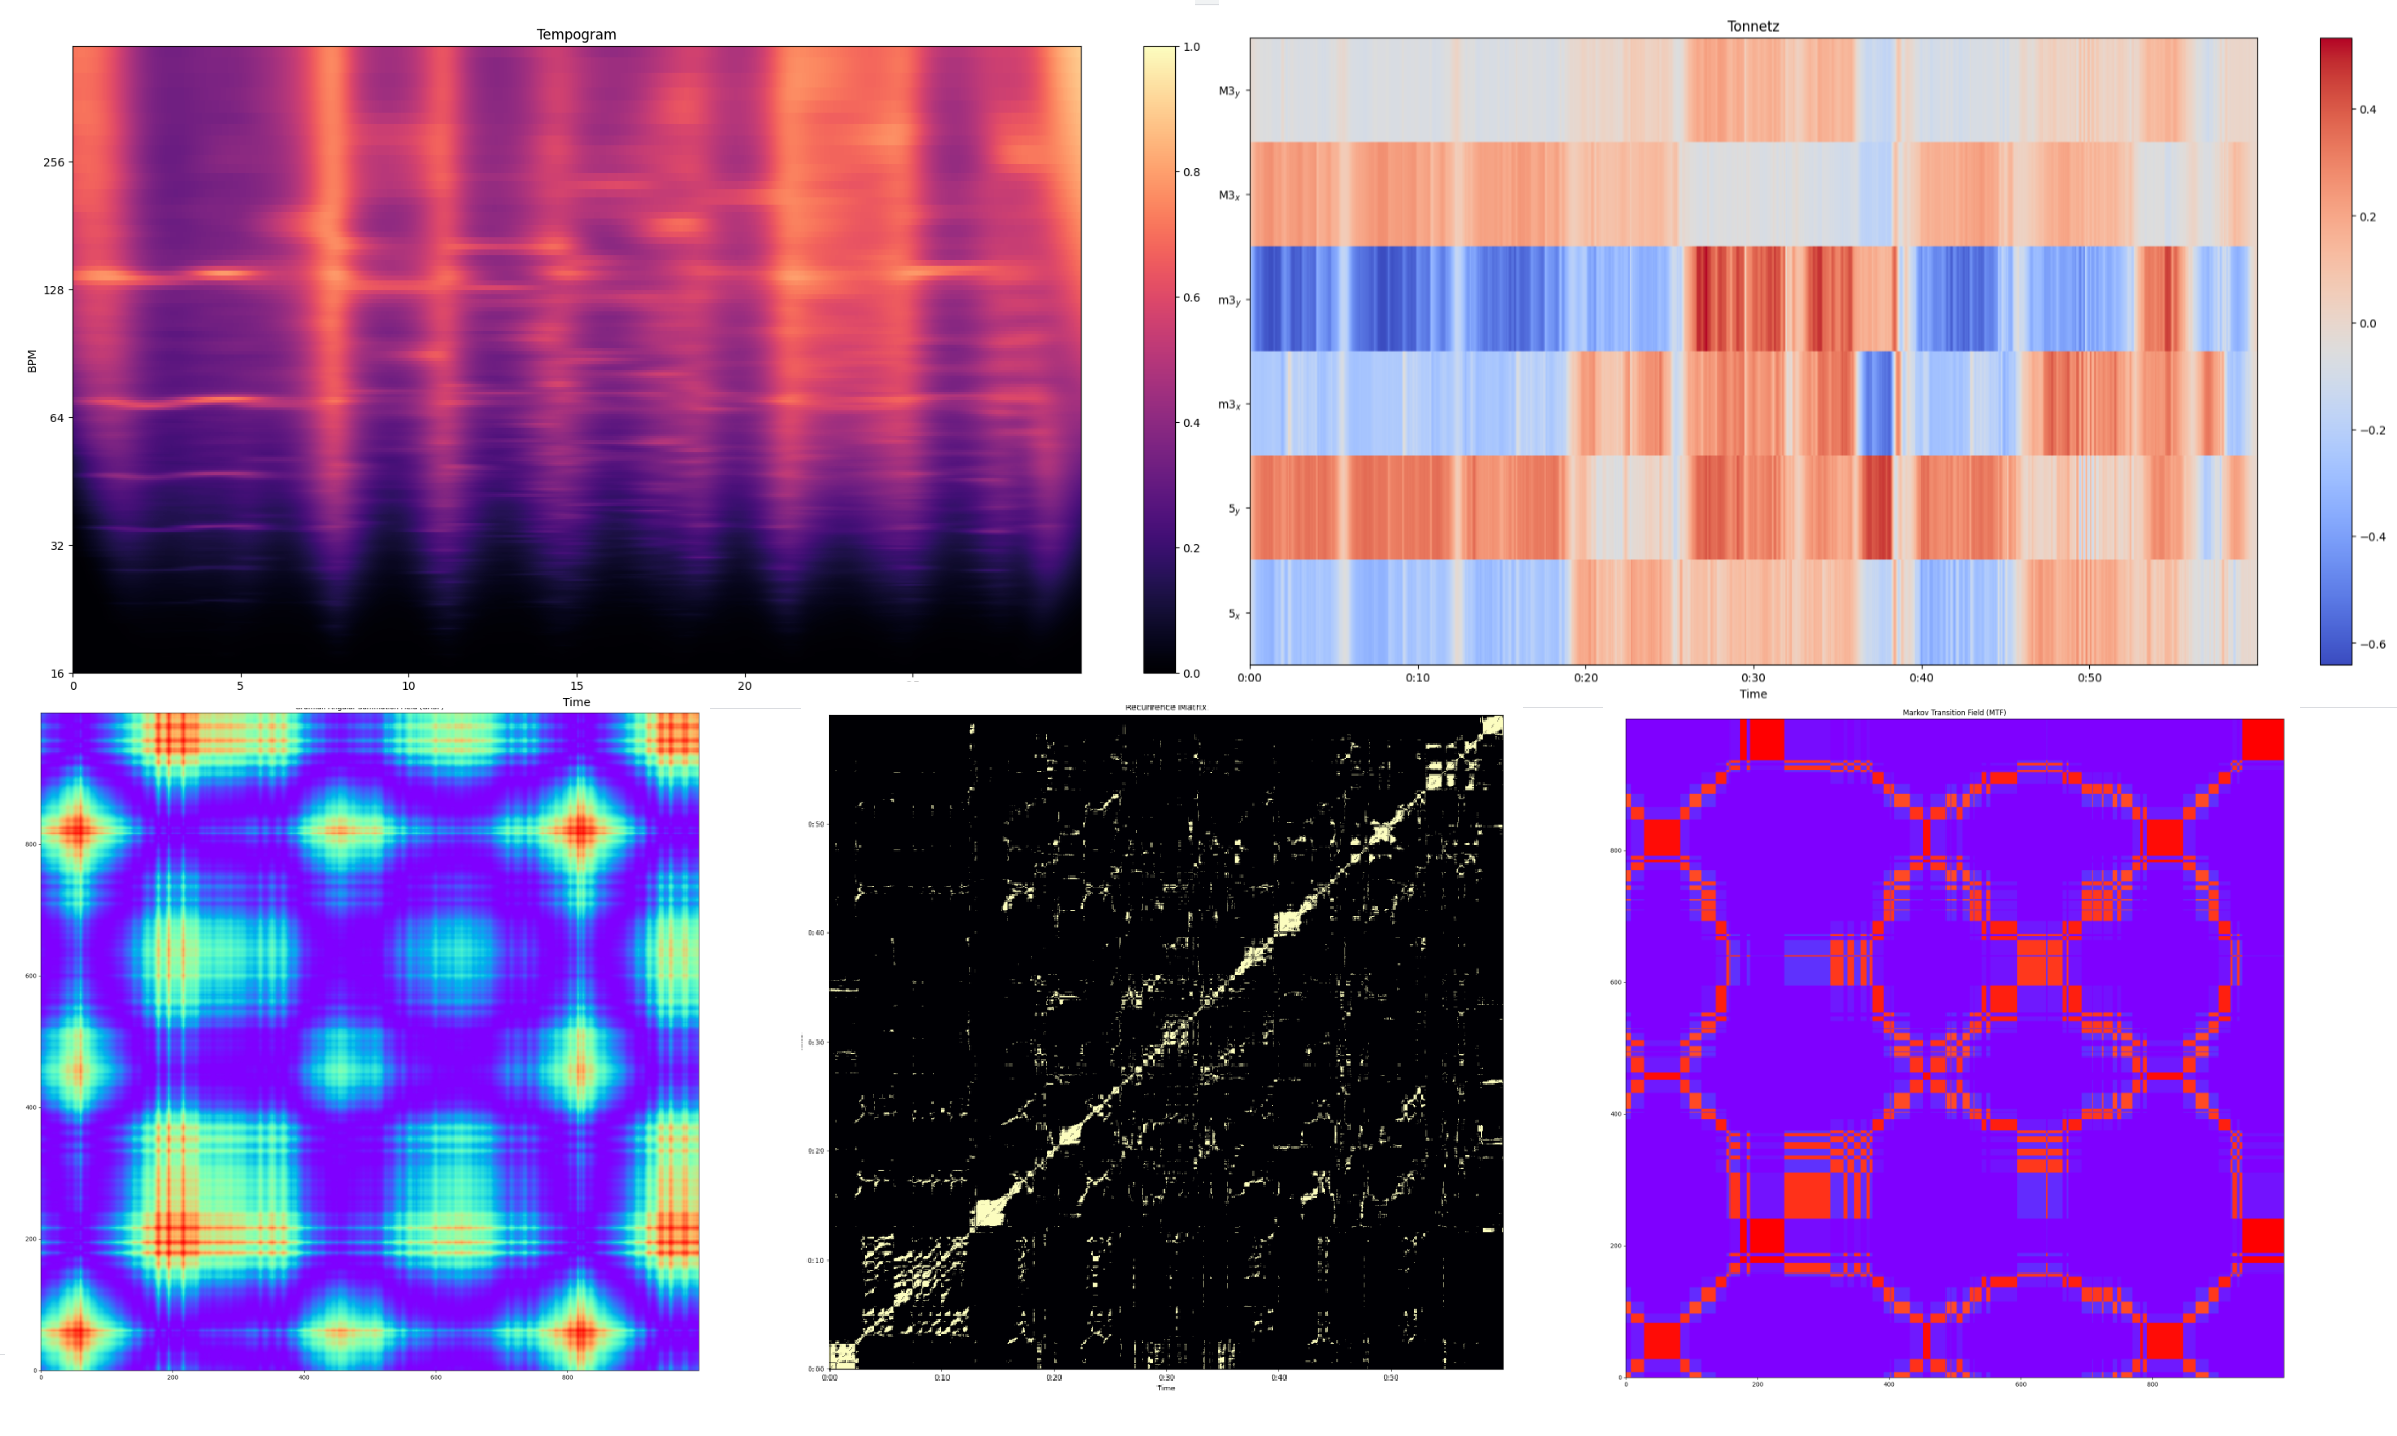
\includegraphics[width=1.2\textwidth]{Different pictures.png}
  
    \label{fig:my_image}
\end{figure}


\end{document}